\chapter{Исследовательская часть}

В данном разделе будут приведены примеры работы программы, и будет проведен сравнительный анализ реализованных алгоритмов умножения матриц по затраченному процессорному времени.

\section{Технические характеристики}

Тестирование проводилось на устройстве со следующими техническими характеристиками:

\begin{itemize}
	\item операционная система: Ubuntu 20.04.1 Linux x86\_64 \cite{linux};
	\item память : 8 GiB;
	\item процессор: AMD® Ryzen™ 3 3200u @ 2.6 GHz \cite{amd}.
\end{itemize}

Тестирование проводилось на ноутбуке, включенном в сеть электропитания. Во время тестирования ноутбук был нагружен только встроенными приложениями окружения, а также непосредственно системой тестирования.

\clearpage

\section{Демонстрация работы программы}

На рисунке \ref{img:example} приведен пример работы программы.

\begin{figure}[H]
	\begin{center}
		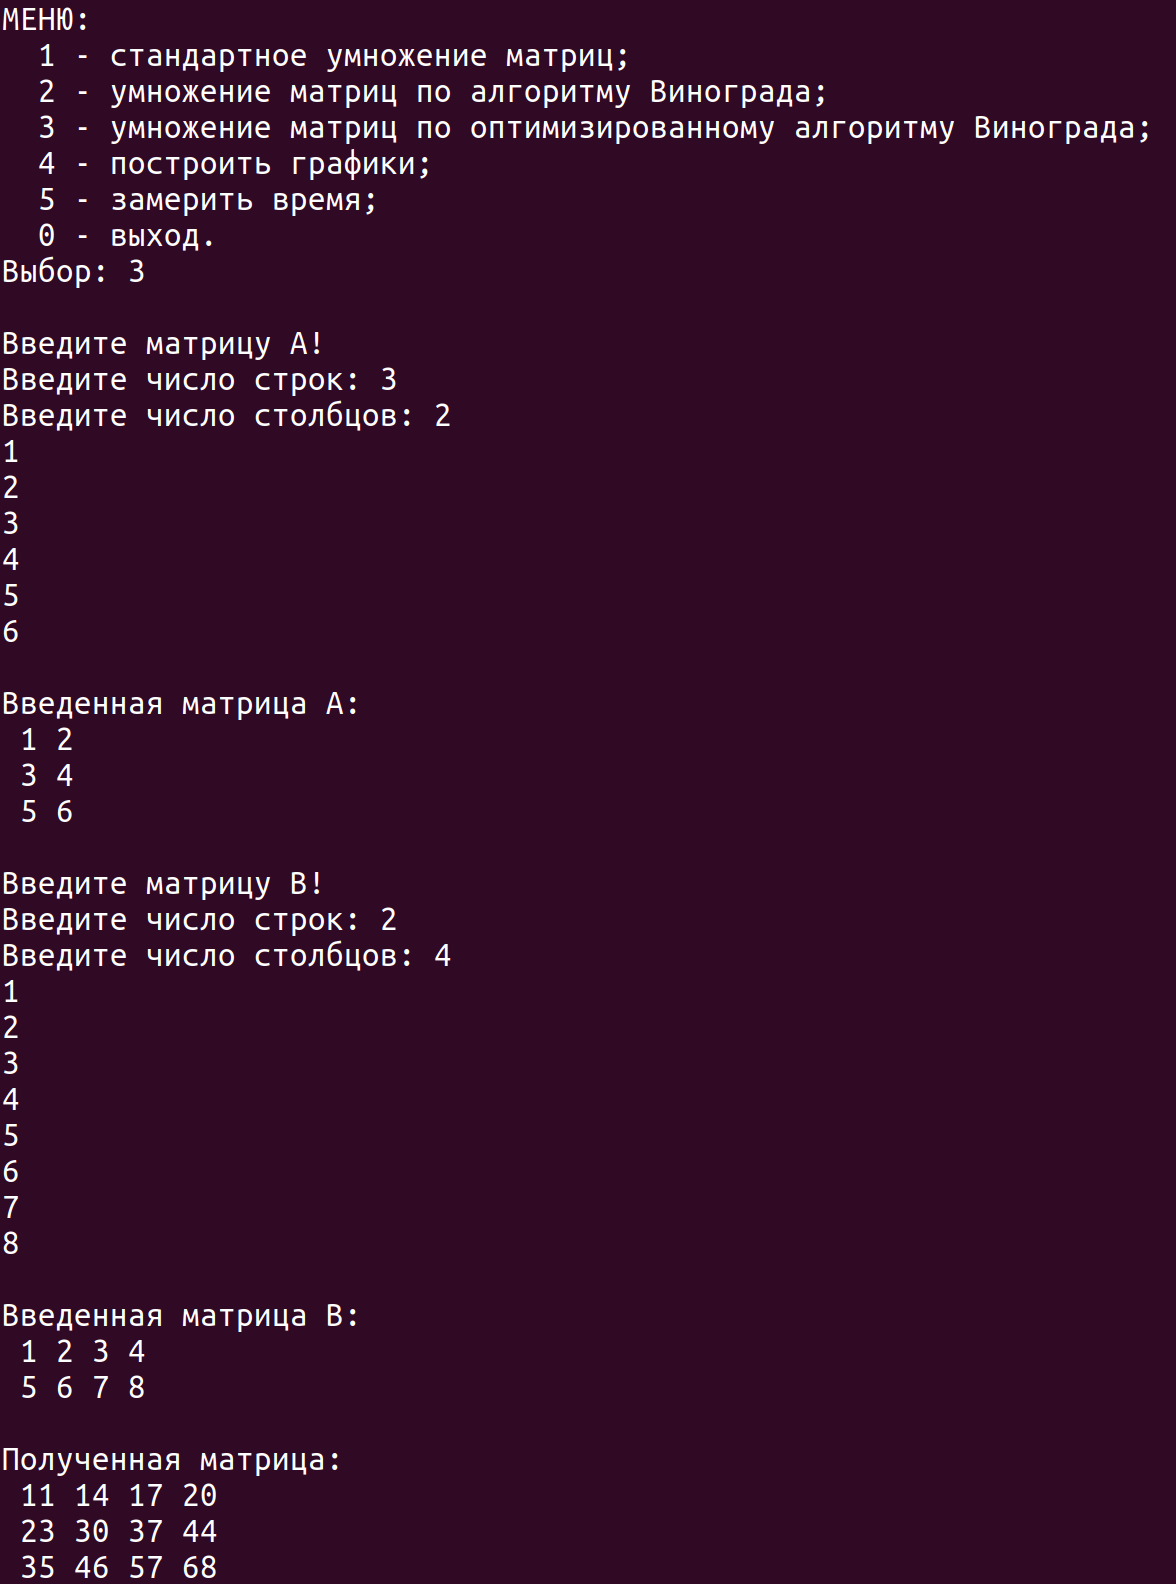
\includegraphics[scale=0.3]{img/example.png}
	\end{center}
	\captionsetup{justification=centering}
	\caption{Пример работы программы}
	\label{img:example}
\end{figure}

\section{Время выполнения алгоритмов}

Функция process\_time из библиотеки time ЯП Python возвращает  процессорное время в секундах - значение типа float.

Для замера времени:
\begin{itemize}
	\item получить значение времени до начала выполнения алгоритма, затем после её окончания. Чтобы получить результат, необходимо вычесть из второго значения первое;
	\item первый шаг необходимо повторить iters раз (в программе iters равно 10), суммируя полученные значения, а затем усреднить результат.
\end{itemize}

Замеры проводились для квадратных матриц целых чисел, заполненных случайным образом, размером от 10 до 100 и от 11 до 101. Результаты измерения времени для четного размера матриц приведены в таблице \ref{tbl:time_even} (в мс).

\begin{table}[h]
    \begin{center}
        \begin{threeparttable}
        \captionsetup{justification=raggedright,singlelinecheck=off}
        \caption{Результаты замеров времени}
        \label{tbl:time_even}
        \begin{tabular}{|c|c|c|c|}
            \hline
            Размер & Стандартный & Винограда & Опт-ый Винограда  \\
            \hline
		    10 & 0.2875 & 0.6851 & 0.2061 \\
			\hline
			20 & 1.6220 & 3.5965 & 1.2381 \\
			\hline
			30 & 5.3519 & 4.4189 & 4.0736 \\
			\hline
			40 & 12.2201 & 9.7817 & 9.0212 \\
			\hline
			50 & 23.4212 & 18.8085 & 18.8640 \\
			\hline
			60 & 39.3355 & 32.1766 & 30.2312 \\
			\hline
			70 & 61.6586 & 52.5354 & 50.6840 \\
			\hline
			80 & 91.7189 & 81.2931 & 73.1704 \\
			\hline
			90 & 129.2349 & 110.4791 & 104.2271 \\
			\hline
			100 & 177.5043 & 158.5571 & 134.2171 \\
			\hline
		\end{tabular}
    \end{threeparttable}
\end{center}
\end{table}

На рисунке \ref{img:even} приведены графические результаты сравнения временных характеристик для четного размера матриц.

\begin{figure}[H]
	\begin{center}
		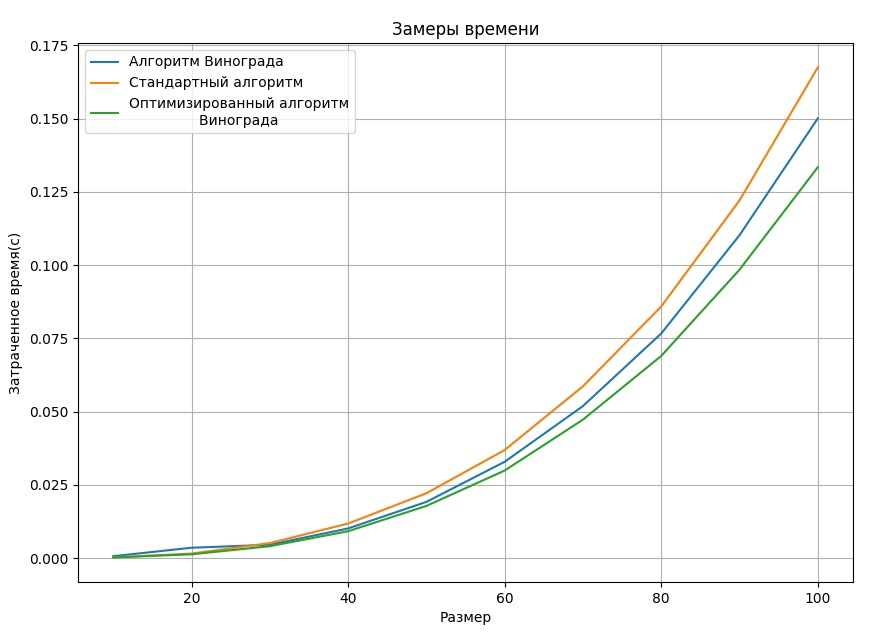
\includegraphics[scale=0.5]{img/even.jpg}
	\end{center}
	\captionsetup{justification=centering}
	\caption{Сравнение по времени алгоритмов умножения матриц четного размера}
	\label{img:even}
\end{figure}

Результаты измерения времени для четного размера матриц приведены в таблице \ref{tbl:time_odd} (в мс).

\begin{table}[h]
    \begin{center}
        \begin{threeparttable}
        \captionsetup{justification=raggedright,singlelinecheck=off}
        \caption{Результаты замеров времени}
        \label{tbl:time_odd}
        \begin{tabular}{|c|c|c|c|}
            \hline
            Размер & Стандартный & Винограда & Опт-ый Винограда  \\
            \hline
			11 & 0.2942 & 0.8884 & 0.2907 \\
			\hline
			21 & 1.8007 & 3.2802 & 1.6107 \\
			\hline
			31 & 5.5211 & 4.6575 & 4.8589 \\
			\hline
			41 & 12.0378 & 10.6847 & 10.6740 \\
			\hline
			51 & 23.3503 & 20.2865 & 19.9010 \\
			\hline
			61 & 41.0413 & 34.2695 & 32.9210 \\
			\hline
			71 & 65.2536 & 54.6966 & 50.5432 \\
			\hline
			81 & 93.8148 & 82.2679 & 72.8342 \\
			\hline
			91 & 131.0258 & 118.6902 & 105.8783 \\
			\hline
			101 & 177.7476 & 158.8673 & 142.5004 \\
			\hline
		\end{tabular}
    \end{threeparttable}
\end{center}
\end{table}

На рисунке \ref{img:odd} приведены графические результаты сравнения временных характеристик для нечетного размера матриц.

\begin{figure}[H]
	\begin{center}
		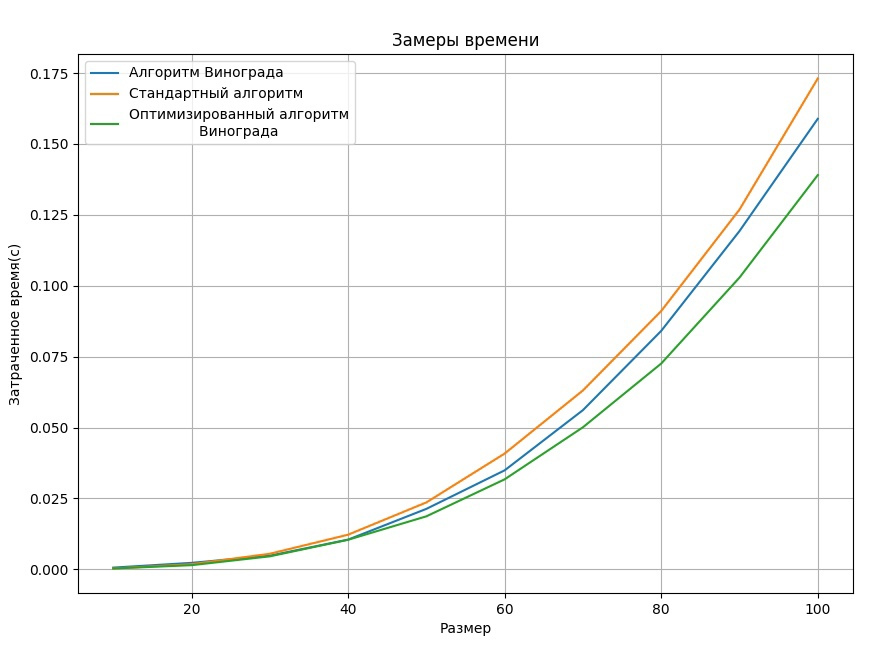
\includegraphics[scale=0.5]{img/odd.jpg}
	\end{center}
	\captionsetup{justification=centering}
	\caption{Сравнение по времени алгоритмов умножения матриц нечетного размера}
	\label{img:odd}
\end{figure}

\section{Вывод}

В результате эксперимента было получено, что при размере матриц, большем 30, оптимизированный алгоритм Винограда работает работает быстрее стандартного алгоритма в 1.3 раза. При этом стандартный алгоритм медленнее алгоритма Винограда в 1.2 раза. Тогда, для размера матриц, начиная с 30 элементов, небходимо использовать оптимизированный алгоритм умножения матриц по Винограду.

Также в результате эксперимента было установлено, что при четном размере матриц, алгоритм Винограда работает быстрее, чем на матрицах с нечетным размером в 1.2 раза в связи с проведением дополнительных вычислений для крайних строк и столбцов. Можно сделать вывод, что алгоритм Винограда предпочтительно использовать для умножения матриц четных размеров.